\documentclass[tikz, border=10pt]{standalone}
\usepackage{tikz}
\usetikzlibrary{shapes.geometric, arrows.meta, positioning, backgrounds}

\definecolor{grucolor}{RGB}{52, 120, 190}
\definecolor{mhacolor}{RGB}{34, 150, 100}
\definecolor{mlpcolor}{RGB}{190, 80, 50}
\definecolor{blockbg}{RGB}{245, 248, 255}
\definecolor{arrowcolor}{RGB}{60, 60, 60}

\tikzset{
  hblock/.style={
    rectangle, rounded corners=5pt,
    minimum width=5.5cm, minimum height=1.0cm,
    draw=gray!40, thick, fill=blockbg
  },
  ioblock/.style={
    rectangle, rounded corners=3pt,
    minimum width=5.5cm, minimum height=0.62cm,
    text centered, font=\small,
    fill=gray!15, draw=gray!50
  },
  arr/.style={-{Stealth[length=5pt]}, thick, color=arrowcolor},
  garr/.style={-{Stealth[length=4.5pt]}, thick, color=grucolor!80}
}

% block height = 1.0cm, node distance = 0.8cm
% center-to-center vertical distance = 0.5 + 0.8 + 0.5 = 1.8cm

\newcommand{\blockinnards}[1]{%
  \node[font=\scriptsize\bfseries, text=grucolor!80!black]
    at ([xshift=-1.6cm]#1.center) {GRU};
  \node[font=\scriptsize, text=gray!40]
    at ([xshift=-0.65cm]#1.center) {|};
  \node[font=\scriptsize\bfseries, text=mhacolor!80!black]
    at (#1.center) {MHA};
  \node[font=\scriptsize, text=gray!40]
    at ([xshift=0.65cm]#1.center) {|};
  \node[font=\scriptsize\bfseries, text=mlpcolor!80!black]
    at ([xshift=1.6cm]#1.center) {MLP};
}

\begin{document}
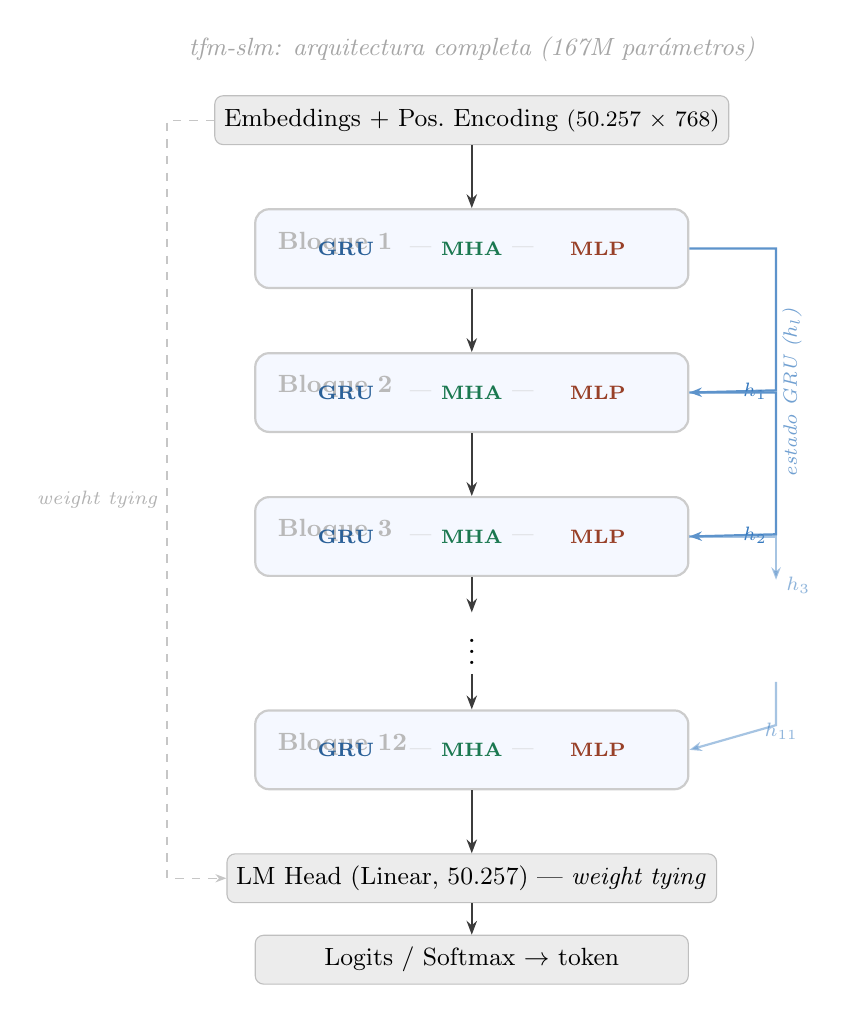
\begin{tikzpicture}[node distance=0.8cm]

  % ── Title ──────────────────────────────────────────────────────
  \node[font=\small\itshape, text=gray!70] (title)
    {tfm-slm: arquitectura completa (167M parámetros)};

  % ── Input ──────────────────────────────────────────────────────
  \node[ioblock, below=0.3cm of title] (embed)
    {Embeddings + Pos.\ Encoding \footnotesize{(50.257 $\times$ 768)}};

  % ── Block 1 ────────────────────────────────────────────────────
  \node[hblock, below=of embed] (b1) {};
  \node[font=\small\bfseries, text=gray!55,
        anchor=north west, xshift=5pt, yshift=-5pt] at (b1.north west) {Bloque 1};
  \blockinnards{b1}

  % ── Block 2 ────────────────────────────────────────────────────
  \node[hblock, below=of b1] (b2) {};
  \node[font=\small\bfseries, text=gray!55,
        anchor=north west, xshift=5pt, yshift=-5pt] at (b2.north west) {Bloque 2};
  \blockinnards{b2}

  % ── Block 3 ────────────────────────────────────────────────────
  \node[hblock, below=of b2] (b3) {};
  \node[font=\small\bfseries, text=gray!55,
        anchor=north west, xshift=5pt, yshift=-5pt] at (b3.north west) {Bloque 3};
  \blockinnards{b3}

  % ── Dots ───────────────────────────────────────────────────────
  \node[font=\large, below=0.45cm of b3] (dots) {$\vdots$};

  % ── Block 12 ───────────────────────────────────────────────────
  \node[hblock, below=0.45cm of dots] (b12) {};
  \node[font=\small\bfseries, text=gray!55,
        anchor=north west, xshift=5pt, yshift=-5pt] at (b12.north west) {Bloque 12};
  \blockinnards{b12}

  % ── Output ─────────────────────────────────────────────────────
  \node[ioblock, below=of b12] (lmhead)
    {LM Head (Linear, 50.257) — \textit{weight tying}};
  \node[ioblock, below=0.4cm of lmhead] (logits)
    {Logits / Softmax $\rightarrow$ token};

  % ── Main flow arrows ────────────────────────────────────────────
  \draw[arr] (embed.south)  -- (b1.north);
  \draw[arr] (b1.south)     -- (b2.north);
  \draw[arr] (b2.south)     -- (b3.north);
  \draw[arr] (b3.south)     -- (dots.north);
  \draw[arr] (dots.south)   -- (b12.north);
  \draw[arr] (b12.south)    -- (lmhead.north);
  \draw[arr] (lmhead.south) -- (logits.north);

  % ── GRU hidden-state channel (right side) ──────────────────────
  % center-to-center = 1.8cm; channel offset = +1.1cm from block east

  % h_1: Block 1 → Block 2
  \draw[garr]
    (b1.east) -- ++(1.1,0) -- ++(0,-1.8) -- (b2.east)
    node[pos=0.5, right, font=\scriptsize\bfseries, text=grucolor] {$h_1$};

  % h_2: Block 2 → Block 3
  \draw[garr]
    (b2.east) -- ++(1.1,0) -- ++(0,-1.8) -- (b3.east)
    node[pos=0.5, right, font=\scriptsize\bfseries, text=grucolor] {$h_2$};

  % h_3 stub going into dots
  \draw[garr, opacity=0.55]
    (b3.east) -- ++(1.1,0) -- ++(0,-0.55)
    node[right, font=\scriptsize\bfseries, text=grucolor, yshift=-2pt] {$h_3$};

  % h_11 stub coming out of dots into b12
  \draw[garr, opacity=0.55]
    ([xshift=1.1cm]b3.east |- dots.south) ++(0,-0.1)
    -- ++(0,-0.55) -- (b12.east)
    node[pos=0.25, right, font=\scriptsize\bfseries, text=grucolor] {$h_{11}$};

  % ── Weight tying annotation (left side) ─────────────────────────
  \draw[dashed, gray!45, -{Stealth[length=4pt]}]
    (embed.west) -- ++(-0.6,0) |- (lmhead.west)
    node[pos=0.25, left, font=\scriptsize\itshape, text=gray!60] {weight tying};

  % ── GRU channel label ───────────────────────────────────────────
  \node[font=\scriptsize\itshape, text=grucolor!70,
        rotate=90, anchor=south]
    at ([xshift=1.55cm]b2.east) {estado GRU ($h_l$)};

\end{tikzpicture}
\end{document}
